\documentclass[]{article}

\usepackage{amsmath}
\usepackage[utf8]{inputenc}
\usepackage[usenames,dvipsnames]{xcolor}
\usepackage{fullpage}
\usepackage[upright]{fourier}
\usepackage{tkz-graph}
\usepackage{color}
\usetikzlibrary{arrows}

\usepackage[paperheight=2.9in,paperwidth=2.7in,margin=0in]{geometry}
\definecolor{color1}{RGB}{251,180,174}
\definecolor{color2}{RGB}{179,205,227}
\definecolor{color3}{RGB}{204,235,197}
\definecolor{color4}{RGB}{222,203,227}

\begin{document}
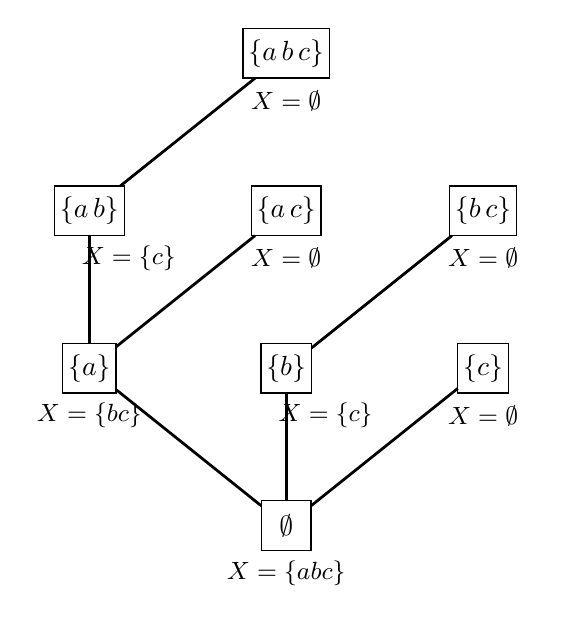
\begin{tikzpicture}
  \SetVertexNormal[Shape     = rectangle,
                   FillColor = white,
                  LineWidth  = 1pt]
  \SetUpEdge[lw         = 1pt,
             color      = black,
             labelcolor = white,
             labeltext  = red,
             labelstyle = {sloped,draw,text=blue}]

% level 0
\SetVertexNormal[Shape = rectangle, FillColor  = white]
\Vertex[x=0, y=0, LabelOut=true, Ldist=5pt]{}
\Vertex[x=0, y=0, L=$\emptyset$]{$000$}

% level 1
\Vertex[x=-2.5, y=2, LabelOut=true, Ldist=5pt]{}
    \Vertex[x=-2.5, y=2, L=$\{a\}$]{$100$}
\Vertex[x=0, y=2, LabelOut=true, Ldist=5pt]{}
    \Vertex[x=0, y=2, L=$\{b\}$]{$010$}
\Vertex[x=2.5, y=2, LabelOut=true, Ldist=5pt]{}
    \Vertex[x=2.5, y=2, L=$\{c\}$]{$001$}

% level 2
\Vertex[x=-2.5, y=4, LabelOut=true, Ldist=5pt]{}
\Vertex[x=-2.5, y=4, L=$\{a\,b\}$]{$110$}
\Vertex[x=0, y=4, LabelOut=true, Ldist=5pt]{}
\Vertex[x=0, y=4, L=$\{a\,c\}$]{$101$}
\Vertex[x=2.5, y=4, LabelOut=true, Ldist=5pt]{}
\Vertex[x=2.5, y=4, L=$\{b\,c\}$]{$011$}

% level 3
\SetVertexNormal[Shape = rectangle, FillColor = white]
\Vertex[x=0, y=6, LabelOut=true, Ldist=5pt]{}
    \Vertex[x=0, y=6, L=$\{a\,b\,c\}$]{$111$}

\tikzset{EdgeStyle/.style={-}}

\SetUpEdge[lw = 1pt, color= black]
\Edges($000$, $100$) 
\Edges($000$, $010$) 
\Edges($000$, $001$) 
\Edges($100$, $101$) 
\Edges($100$, $110$) 
\Edges($010$, $011$) 
\Edges($110$, $111$) 

\node[] at (0,-.6) 
    {\small $X = \{a b c\}$};
\node[] at (-2.5, 1.4) 
    {\small $X = \{b c\}$};
\node[] at (.5, 1.4) 
    {\small $X = \{c\}$};
\node[] at (2.5, 1.4) 
    {\small $X = \emptyset$};
\node[] at (2.5, 3.4) 
    {\small $X = \emptyset$};
\node[] at (0, 3.4) 
    {\small $X = \emptyset$};
\node[] at (-2., 3.4) 
    {\small $X = \{c\}$};
\node[] at (0, 5.4) 
    {\small $X = \emptyset$};
\end{tikzpicture}
\end{document}
